\documentclass[10pt]{article}
\usepackage[margin=0.9in]{geometry}
\usepackage{graphicx}
\usepackage{booktabs}
\usepackage{longtable}
\usepackage{amsmath}
\usepackage{float}
\usepackage[hidelinks]{hyperref}
\usepackage{caption}
\usepackage[numbers,square,sort&compress]{natbib}
\usepackage{microtype}
\graphicspath{{figures/}}
% Generated by scripts/analysis/exponential_bootstrap.py. Do not edit.
\newcommand{\betaQM}{0.328}
\newcommand{\sigQM}{0.014}
\newcommand{\nQM}{231}
\newcommand{\loQM}{0.302}
\newcommand{\hiQM}{0.358}
\newcommand{\betaEM}{0.354}
\newcommand{\sigEM}{0.010}
\newcommand{\nEM}{450}
\newcommand{\loEM}{0.332}
\newcommand{\hiEM}{0.372}
\newcommand{\betaWaves}{0.348}
\newcommand{\sigWaves}{0.015}
\newcommand{\nWaves}{167}
\newcommand{\loWaves}{0.314}
\newcommand{\hiWaves}{0.371}
\newcommand{\betaMechanics}{0.369}
\newcommand{\sigMechanics}{0.018}
\newcommand{\nMechanics}{154}
\newcommand{\loMechanics}{0.314}
\newcommand{\hiMechanics}{0.386}
\newcommand{\betaThermo}{0.399}
\newcommand{\sigThermo}{0.017}
\newcommand{\nThermo}{96}
\newcommand{\loThermo}{0.367}
\newcommand{\hiThermo}{0.435}
\newcommand{\betaFluid}{0.406}
\newcommand{\sigFluid}{0.024}
\newcommand{\nFluid}{54}
\newcommand{\loFluid}{0.359}
\newcommand{\hiFluid}{0.457}
\newcommand{\simCrit}{3.11}
\newcommand{\nExclude}{1}
\newcommand{\bootN}{10000}
\newcommand{\bootSeed}{8888}
\newcommand{\betaFeynBench}{0.342}
\newcommand{\sigFeynBench}{0.013}
\newcommand{\nFeynBench}{100}
\newcommand{\loFeynBench}{0.319}
\newcommand{\hiFeynBench}{0.371}
\newcommand{\betaFeynAll}{0.354}
\newcommand{\sigFeynAll}{0.009}
\newcommand{\nFeynAll}{1016}
\newcommand{\loFeynAll}{0.332}
\newcommand{\hiFeynAll}{0.366}
\newcommand{\betaWiki}{0.314}
\newcommand{\sigWiki}{0.015}
\newcommand{\nWiki}{76}
\newcommand{\loWiki}{0.284}
\newcommand{\hiWiki}{0.344}
\newcommand{\betaEI}{0.267}
\newcommand{\sigEI}{0.010}
\newcommand{\nEI}{70}
\newcommand{\loEI}{0.252}
\newcommand{\hiEI}{0.291}
\newcommand{\betaLeemis}{0.269}
\newcommand{\sigLeemis}{0.014}
\newcommand{\nLeemis}{61}
\newcommand{\loLeemis}{0.250}
\newcommand{\hiLeemis}{0.305}
\newcommand{\betafR}{0.270}
\newcommand{\sigfR}{0.021}
\newcommand{\nfR}{37}
\newcommand{\lofR}{0.265}
\newcommand{\hifR}{0.347}
\newcommand{\betaPooled}{0.354}
\newcommand{\sigPooled}{0.009}
\newcommand{\nPooled}{1016}
\newcommand{\nLabelled}{967}
\newcommand{\nFeynAllExpr}{1016}
\newcommand{\nLectAdded}{916}

% \input is not expandable inside tabular; the TeX primitive is.
\makeatletter\newcommand{\tabinput}[1]{\@@input #1 }\makeatother

\title{Branch-Dependent Priors for Symbolic Regression in Physics}
% TODO(author): author name and affiliation (Chun Hin Ma?). Not filled in on purpose.
\author{}
\date{}

\begin{document}
\maketitle

\begin{center}
\small\itshape Work in progress. This write-up is still being updated.
\end{center}

\begin{abstract}
Bayesian symbolic regression uses a prior to express which equation forms are plausible before considering the data, and such a prior can be learned from a curated collection of scientific equations. In physics, ranked operator frequencies have been found to decline more slowly in a collection of inflationary potentials than in broader physics collections. This raises the question of whether physics equations have different statistical signatures across domains, which might explain the difference in decay rates. We revisit the gap using direct log least squares, a computationally simpler approach than training a simulation-based estimator. The gap persists after changes to constant conventions. To analyse a larger collection of expressions, we expand the Feynman collection to about 1,000 expressions, with 967 assigned to seven branches. We also build a corpus of 37 expressions for proposed $f(R)$ modified-gravity models and include 76 formulas from Wikipedia's list of scientific equations named after people and 70 potentials from Encyclopaedia Inflationaris. We created a public formula ledger for searching expressions, tracing their sources, inspecting expression trees and operator counts, and exploring plots of decay rate against complexity. We estimate exponential decay rates and nominal 95\% bootstrap intervals for the collections and branches. The estimates suggest that the decay rate varies across branches of physics. Variation in operator use motivates asking whether adapting a symbolic regression prior to a specific branch gives more probability to the functional forms of equations from that branch. We test this using grouped six-fold cross-validation on 943 branch-labelled Feynman formulas. The pooled prior learns operator arrangements from training formulas across all branches, and the branch-dependent prior adjusts those probabilities using the subset of those training formulas from the relevant branch. We compare the probabilities the two priors assign to each held-out expression tree. The branch-dependent prior assigns 1.34 times as much probability as the pooled prior on a geometric-average basis. It assigns higher probabilities on average in six of the seven branches, suggesting that branch information helps describe equation forms within the fields studied.
\end{abstract}

\section{Introduction}
Symbolic regression searches for equations that explain observations and make testable predictions. In Bayesian symbolic regression, a prior expresses which equation forms are plausible before considering the data. These preferences can be learned from existing equations. Guimer\`a et al. constructed a prior from operator counts in 4,080 mathematical expressions collected from Wikipedia. Bartlett et al. trained a language model on 161 scientific equations to learn how operators are arranged within expression trees~\citep{guimera2020,bartlett2023}.

Constantin et al. found that the ranked frequencies of mathematical operators in physics equations follow an approximate exponential decay law, which they call a meta-law. This is analogous to Zipf's law in natural language, where word frequencies decline with rank according to a power law. They represented each expression as a tree, counted occurrences of each operator type, and ranked the types from most to least frequent. The fitted law has the form
\[
f(r)\propto e^{-\beta r},
\]
where $f(r)$ is the frequency at rank $r$ and $\beta$ is the decay rate~\citep{constantin2026}.

At $\beta=0$, all operator types in the fit have the same frequency. At large $\beta$, most occurrences are concentrated among the few most frequent types. Constantin et al. found decay rates of about $\beta=1/3$ for the Feynman benchmark, the Wikipedia equations and the \textit{Cambridge Handbook of Physics Formulas}. The potentials in \textit{Encyclopaedia Inflationaris} had a lower decay rate of about $\beta=1/4$. The three broader collections bring together equations from several branches of established physics. \textit{Encyclopaedia Inflationaris} collects proposed potentials for single-field slow-roll inflation. Its expressions describe a single physical quantity in a speculative area of high-energy cosmology and are written using natural units~\citep{constantin2026,martin2014}.

We revisit the gap to examine whether a common decay rate can describe equations across physics, a question that informs whether we should build one prior for physics or adapt it to individual branches. We estimate the decay rate by least squares on the log frequencies and estimate uncertainty by resampling whole equations. This computationally simpler procedure gives rates close to the published simulation-based estimates for the Feynman benchmark and the inflationary potentials and reproduces the gap between them~\citep{constantin2026}.

To make the comparisons reproducible and support further analysis, we curate a catalogue that includes the 100-expression Feynman benchmark, 76 equations from Wikipedia, 70 inflationary potentials and 37 expressions for proposed $f(R)$ gravity models. We expand the Feynman benchmark with formulas from all three volumes of \textit{The Feynman Lectures on Physics}, bringing the collection to about 1,000 expressions, of which 967 are assigned to seven physics branches~\citep{udrescu2020,feynman}. We make the catalogue available in a \href{https://jaysen-ma.github.io/physics-priors/data/catalog/index.html}{public formula ledger} where readers can search expressions, trace their sources, inspect expression trees and operator counts, and explore plots of decay rate against expression complexity.

We first examine whether the gap is sensitive to constant conventions. Setting $c=\hbar=1$ where applicable and removing the common amplitude prefactor from the inflationary potentials changes the gap with the Feynman benchmark very little. The $f(R)$ collection, another set of proposed forms for a single physical quantity, gives a similarly low fitted rate~\citep{sotiriou2010}. With 37 expressions, its bootstrap interval is wide enough to span both the inflationary and Feynman benchmark estimates. The comparison leaves the cause of the gap open.

Constantin et al. also suggested that $\beta$ could vary with energy scale~\citep{constantin2026}. The three broader collections pool equations from several fields, so fitting a single rate to each collection may obscure differences between its constituent branches. We therefore estimate the decay rate separately for seven physics branches in the expanded Feynman collection. The estimates suggest some variation, with higher fitted rates for thermodynamics and kinetic theory and for fluid and continuum mechanics than for electromagnetism or quantum mechanics.

This variation motivates building a prior for a new symbolic regression task that is adapted to its known physics branch. We compare a pooled prior that learns operator arrangements across all training branches with a branch-dependent prior that adjusts those probabilities using the relevant branch's subset of the same training formulas.

We evaluate both priors on 943 branch-labelled Feynman formulas using grouped six-fold cross-validation. We keep equivalent and related formulas together and compare the probabilities the two priors assign to each held-out expression tree. On a geometric-average basis, the branch-dependent prior assigns 1.34 times as much probability as the pooled prior. The ratio exceeds one in six of the seven branches, suggesting that branch information helps describe equation forms in the Feynman collection.

Section~\ref{sec:data} describes the sources of the equation catalogues and how we selected expressions. It explains how we assigned Feynman formulas to physics branches and what the public formula ledger records. Section~\ref{sec:decay} explains how we estimate exponential decay rates and their uncertainty. We revisit the inflationary gap and compare the fitted rates across the seven Feynman branches. Section~\ref{sec:priors} describes how a pooled prior learns operator arrangements in expression trees. We then use the relevant branch's subset of the same training formulas to adapt that prior. Section~\ref{sec:prior-evaluation} describes the grouped six-fold evaluation on held-out formulas. It reports how much probability the branch-dependent prior assigns relative to the pooled prior, both overall and within each branch. Section~\ref{sec:discussion} discusses what the decay-rate and prior comparisons tell us about the structure of physics equations. It considers how these findings might inform symbolic regression and what remains to be tested.

\section{Equation catalogues}\label{sec:data}

\subsection{Sources and coverage}
We curate a source-linked catalogue of mathematical expressions for inspection and reuse. It includes the \nFeynBench{} expressions in the AI Feynman benchmark, \nWiki{} formulas from entries in Wikipedia's \textit{List of scientific equations named after people}, and \nEI{} inflaton potentials from \textit{Encyclopaedia Inflationaris}~\citep{constantin2026,udrescu2020,wikinamed,martin2014}. Each entry records the expression and a reference to its source.

We expand the AI Feynman benchmark with expressions from all three volumes of \textit{The Feynman Lectures on Physics}~\citep{feynman}. After selection and deduplication, we add \nLectAdded{} expressions, comprising 278 from Volume~I, 442 from Volume~II and 196 from Volume~III. The expanded Feynman collection contains \nFeynAll{} expressions.

The modified-gravity catalogue contains \nfR{} proposed curvature functions. It includes 16 variants of one template from P\'erez-Romero and Nesseris~\citep{sotiriou2010,perezromero2018}. We record these variants as a single family and use that grouping to assess how sensitive the fitted decay rate is to including several forms of the same template. Appendix~\ref{app:catalogue} lists the transcription sources.

As a mathematical comparison, we also estimate the decay rate for \nLeemis{} probability density and mass functions from the univariate distributions documented by Leemis and McQueston~\citep{leemis2008}.

\subsection{Expression selection and representation}
For the Feynman Lectures additions, we select equations that give one quantity explicitly in terms of other quantities. We record the quantity on the left-hand side and analyse the expression on the right-hand side. We exclude right-hand sides that consist of a single symbol or number or contain derivatives, integrals, explicit summations, limits or unevaluated quantum-mechanical operators.

We follow the expression-tree representation and operator-counting conventions of Constantin et al. The counting scheme treats variables, numerical literals, and physical or mathematical constants as distinct types of leaves. Sections~II and~III of their paper give the operator definitions and describe the tree representation~\citep{constantin2026}.

\subsection{Branch labels}
After extracting expressions from the three volumes of \textit{The Feynman Lectures on Physics} and combining them with the AI Feynman benchmark, we use Codex with \texttt{gpt-6.2-sol} to assign branch labels to each expression. Codex uses the formula, the quantity it describes and its source context. An expression can receive more than one label. For example, a Lorentz transformation of an electric field can be labelled both electromagnetism and special relativity.

We consider seven physics branches covering classical mechanics, special relativity, electromagnetism, waves and optics, thermodynamics and kinetic theory, quantum mechanics, and fluid and continuum mechanics. We record separate categories for expressions outside these branches and flag unresolved cases. Of the \nFeynAll{} expressions, 967 receive at least one of the seven branch labels and 221 receive more than one. The collection-wide decay-rate fit counts each expression once. Each branch fit includes every expression carrying that branch's label.

\subsection{Formula ledger}
The \href{https://jaysen-ma.github.io/physics-priors/data/catalog/index.html}{public formula ledger} lets readers search the catalogues, follow links to the sources, inspect expression trees and operator counts, and explore plots of decay rate against expression complexity. Lecture entries identify the volume, chapter and equation where available. We also release the formula catalogue, the Codex branch labels and the fold assignments used to keep related formulas together in the prior evaluation.

\section{Variation in operator-frequency decay rates}\label{sec:decay}

\subsection{Estimating the decay rate}\label{sec:methods}
For each collection or branch, we count occurrences of every operator type and arrange the positive counts in descending order,
\[
n_1\geq n_2\geq\cdots\geq n_R>0.
\]
The observed frequency at rank $r$ is
\[
f_r=\frac{n_r}{N},
\qquad N=\sum_{r=1}^{R}n_r.
\]
We model the frequencies by a normalised exponential with decay rate $\beta$:
\begin{equation}
p_r(\beta)=\frac{e^{-\beta r}}{\sum_{s=1}^{R} e^{-\beta s}}.
\label{eq:law}
\end{equation}
Larger values of $\beta$ correspond to frequencies more concentrated at the highest ranks. This model arises as a limit of the two-parameter Zipf--Mandelbrot distribution, as shown in Appendix~\ref{app:zipf-limit}. We fit the exponential directly to each collection, including the Leemis comparison, by minimising the squared differences between observed and model log frequencies:
\begin{equation}
Q(\beta)=\sum_{r=1}^{R}\left[\log f_r-\log p_r(\beta)\right]^2.
\label{eq:logls}
\end{equation}
Each observed rank receives equal weight in this criterion. We include every operator type with a positive count. Types absent from a collection are omitted because their log frequencies are undefined.

The ranking is constructed separately for each collection or branch. Consequently, both the number of observed types and the operator occupying a particular rank can differ between groups. The fitted rate $\hat\beta$ summarises how concentrated each ranked distribution is; it does not describe which operators are most common.

We constrain the numerical optimisation to $0\leq\beta\leq5$ and flag fits near either boundary. Calculating this fitted summary does not require operator occurrences within an equation to be independent. The assumptions needed to interpret its uncertainty enter through the resampling procedure below.

\subsubsection{Uncertainty from equation resampling}
We estimate uncertainty by resampling whole equations. For a collection-wide fit, we draw as many equations as the collection contains, with replacement. For the branch fits, we draw from the 967 branch-labelled formulas. Each selected formula contributes to all branches it belongs to, so the same draw is shared across branches. The number of formulas in each branch can vary between replicates.

For each sample, we recount the operators, determine which types are present, rank their frequencies and refit $\beta$. Repeating this procedure \bootN{} times gives a distribution of fitted rates. We report the fit to the original collection, the standard deviation of the bootstrap estimates as a standard error, and their 2.5th and 97.5th percentiles as an individual 95\% bootstrap interval.

Resampling whole equations keeps together the operators that occur within each expression. Interpreting the resulting intervals as sampling uncertainty assumes that the equations are sufficiently independent and represent a wider collection of comparable expressions. Related equations or variants of the same model can limit this assumption. The intervals also do not account for systematic omissions or transcription errors in the collections.

The reported intervals have a nominal level of 95\%. Appendix~\ref{app:calibration} repeats the procedure on artificial collections with a known decay rate and finds that the resulting intervals contain it less often than 95\% of the time in the cases studied.

We also resample whole source chapters to examine dependence among equations from the same chapter. This check, together with alternative branch assignments and selection rules, is described in Appendix~\ref{app:sensitivity}.

For reproducibility, we use random seed \bootSeed{} and calculate percentiles by linear interpolation (Hyndman--Fan type~7). Failed and degenerate fits are recorded, and intervals affected by missing fits are marked unresolved.

\subsection{Revisiting the inflationary gap}\label{sec:ei}

\subsubsection{Comparison with the published estimates}
We first examine whether the lower decay rate reported for Encyclopaedia Inflationaris is reproduced using the procedure above. Figure~\ref{fig:main} places the Feynman benchmark and inflationary estimates alongside the other physics comparisons. Appendix~\ref{app:sensitivity} gives the complete set of estimates.

The Feynman benchmark gives a fitted rate of $\hat\beta=\betaFeynBench$, with an individual 95\% bootstrap interval of $[\loFeynBench,\hiFeynBench]$. Encyclopaedia Inflationaris gives $\hat\beta=\betaEI$, with an interval of $[\loEI,\hiEI]$. The point estimates differ by 0.075, and their individual intervals do not overlap. The lower inflationary estimate is therefore reproduced with log least squares and equation resampling.

A lower decay rate corresponds to a slower decline in frequency with rank. Under the fitted exponential model, operator occurrences are therefore less concentrated among the most frequent types in the inflationary collection than in the Feynman benchmark. The Leemis collection of probability distributions also gives a fitted rate of $\betaLeemis$. The decay rate is a summary that can be compared across both mathematical and physical collections.

\subsubsection{Changes to constant conventions}\label{sec:units}
One proposed explanation concerns the conventions used to write the equations. Physical constants and amplitude prefactors contribute to the expression trees, so removing them can change the operator counts and the fitted decay rate. We examine two such changes.

First, we set $c=\hbar=1$ in the textbook expressions. This affects 32 expressions in the Feynman benchmark and lowers its fitted rate from 0.342 to 0.332. Two expressions in the Wikipedia collection are affected, and its rate changes by less than 0.001.

Second, we remove the common amplitude prefactor $M^4$ from the inflationary potentials by setting $M=1$. This affects all 70 potentials and lowers the fitted rate from 0.267 to 0.259.

After both changes, the difference between the Feynman benchmark and the inflationary collection is 0.072, compared with 0.075 before the changes. These conventions therefore account for little of the observed difference in point estimates. Other choices of algebraic representation may also affect operator counts, but they are not examined in this comparison.

\subsubsection{Comparison with modified gravity}\label{sec:fr}
We next consider the proposed explanations involving the inflationary collection's focus on one physical concept and its inclusion of hypothetical models. The $f(R)$ gravity collection shares these features: its expressions are proposed forms of a curvature function entering the gravitational action.

The \nfR{} modified-gravity expressions give a fitted rate of $\hat\beta=\betafR$, with an individual 95\% bootstrap interval of $[\lofR,\hifR]$. Its point estimate is close to the inflationary value of $\betaEI$, and the intervals overlap. A similarly low fitted rate is therefore found in another collection of hypothetical models centred on one physical concept.

This similarity does not establish why the rates are close. Both features change together in the comparison, so their effects cannot be distinguished. The modified-gravity collection also contains related variants of model families. These variants influence the operator frequencies and limit the independence assumption underlying equation resampling.

Together, the comparisons reproduce the lower inflationary estimate and show that it changes little relative to the Feynman benchmark under the tested constant conventions. The modified-gravity collection provides a further example of a similar fitted rate, while leaving its explanation unresolved. We next examine variation across physics branches within the expanded Feynman collection.

\subsection{Variation across Feynman branches}\label{sec:results}

The original study proposed differences in energy scale as one possible explanation for the lower inflationary decay rate~\citep{constantin2026}. Inflation also concerns a different branch of physics from much of the material in the broader equation collections. This motivates us to examine whether fitted decay rates vary across physics branches. We use the expanded Feynman collection because the expressions in the Feynman Lectures are publicly accessible~\citep{feynman}. Branch labels provide a way to explore variation with physical domain, although they do not isolate the effect of energy scale.

The fitted rates range from 0.333 in quantum mechanics to 0.445 in special relativity (Figure~\ref{fig:main}). Thermodynamics and kinetic theory and fluid and continuum mechanics have fitted rates of 0.399 and 0.406, respectively. Both are above the estimates for electromagnetism, waves and optics, and classical mechanics. The individual bootstrap intervals overlap across several branches, and the interval for special relativity is especially wide. Figure~\ref{fig:main} also shows five comparison collections.

\begin{figure}[H]\centering
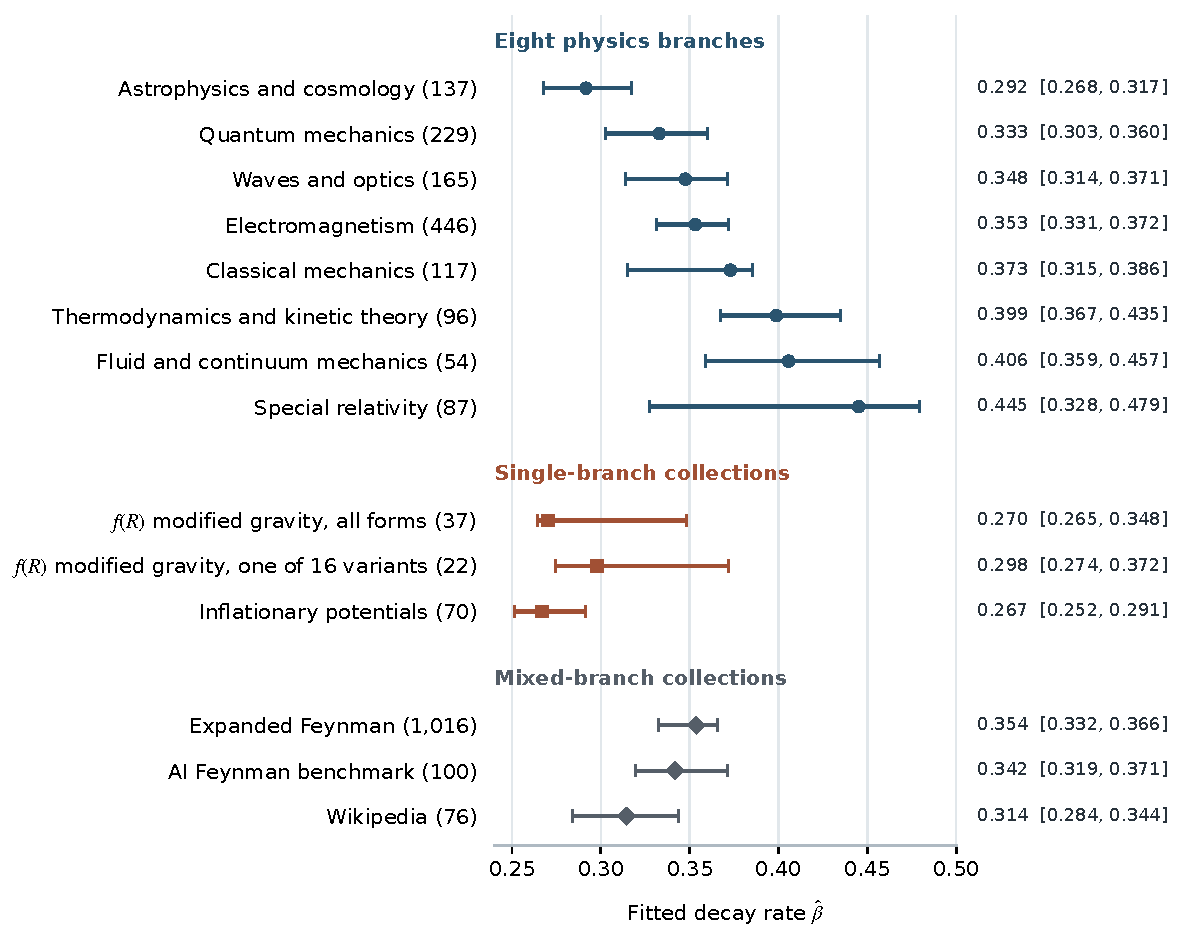
\includegraphics[width=0.8\linewidth]{beta_by_branch.pdf}
\caption{Fitted rates for the seven Feynman branches (circles) and five comparison collections (diamonds, below the dividing line), with nominal individual 95\% equation-bootstrap intervals. The comparison collections are the 100-expression Feynman benchmark, the full expanded Feynman collection, $f(R)$ gravity, Encyclopaedia Inflationaris and Wikipedia. The benchmark is contained in the expanded collection, whose expressions also supply the branch estimates.}\label{fig:main}
\end{figure}

Resampling source chapters widens the intervals for some branches, including quantum mechanics and fluid and continuum mechanics. Appendix~\ref{app:sensitivity} also compares the fitted rates when we use only each formula's primary label or change which equations are included.

The variation in operator frequencies motivates testing whether branch labels also help describe the arrangement of operators in individual expressions.

\section{Learning branch-dependent expression priors}\label{sec:priors}

\subsection{Expression trees and the pooled prior}
We follow Bartlett et al.~\citep{bartlett2023} in treating an expression tree as a sequence of choices about which token occupies each node. We map the selected formulae to a common set of operators and anonymise the leaves, while preserving whether adjacent sibling leaves are identical. For an encoded formula $g$, a model assigns a conditional probability to the token $t_v$ at each node $v$ given its context $h_v$. The score of the whole tree is
\begin{equation}
P(g)=\prod_{v\in g} p(t_v\mid h_v).
\label{eq:tree-score}
\end{equation}
For example, a context can describe the parent operator and which side of it the node occupies. The Katz back-off model uses shorter contexts when more specific ones have insufficient observations. The pooled prior $P_{\mathrm{pool}}$ fits this model across all training branches and blends its probabilities with pooled counts from deeper tree contexts.

\subsection{Branch-dependent adjustment}
For a formula from branch $d$, we start from the pooled prior and fit adjustments using the relevant branch's subset of the same training formulas. The components include adjustments to how often operators with different numbers of children occur, which operator occurs within an arity, and how preferences change with depth or parent operator. One component, $P_{\mathrm{geom},d}$, adjusts the deeper pooled probabilities using the relative frequencies learned from the branch and pooled training formulas. We combine the component scores at the level of whole equations:
\begin{equation}
P_d(g)
=0.75\sum_{m} w_{d,m}P_{d,m}(g)+0.25P_{\mathrm{geom},d}(g).
\label{eq:branch-prior}
\end{equation}
The sum includes the pooled model among its components. The nonnegative mixture weights $w_{d,m}$ sum to one. We learn the weights within the training set. Appendix~\ref{app:prior-fitting} describes the geometric adjustment and weight fitting.

\section{Evaluating priors on held-out equations}\label{sec:prior-evaluation}

\subsection{Grouped cross-validation}
We use a fixed evaluation subset of 943 branch-labelled Feynman expressions and divide them into six folds. We group expressions using known formula families, identified algebraic matches and source-section information. We assign each group to a single fold before constructing any branch-specific training sets. Every label attached to an expression follows it into the same fold.

We hold out each fold in turn. The pooled prior uses each training expression once. Each branch adjustment uses the subset of those expressions carrying its label, so an expression can contribute to more than one branch adjustment. We remove training expressions whose tree encoding is identical to one in the corresponding evaluation set. We apply this check both to the outer test folds and to the three inner validation folds used to learn the mixture weights.

\subsection{Probability ratios}
For held-out expression $g_i$, let $B_i$ be its set of branch labels. Let $P_b(g_i)$ and $P_{\mathrm{pool}}(g_i)$ be the probabilities assigned by the branch-$b$ and pooled priors, both fitted on the corresponding training set. We first average the log probability ratios across the expression's labels,
\begin{equation}
\Delta_i=\frac{1}{|B_i|}\sum_{b\in B_i}
  \log\!\left(\frac{P_b(g_i)}{P_{\mathrm{pool}}(g_i)}\right).
\label{eq:formula-log-ratio}
\end{equation}
We then average across the $N$ held-out expressions and exponentiate,
\begin{equation}
R=\exp\!\left(\frac{1}{N}\sum_{i=1}^{N}\Delta_i\right).
\label{eq:prior-ratio}
\end{equation}
This gives each expression the same weight in the overall comparison. Within each branch, we take the geometric mean of the ratios from that branch's prior for the held-out expressions carrying its label.

\subsection{Preliminary results}
Across the 943 held-out expressions, the geometric mean probability ratio for the branch-dependent prior relative to the pooled prior is 1.34 (Table~\ref{tab:prior-ratios}). The ratio exceeds one in six of the seven branches. For waves and optics it is 0.97.

\begin{table}[H]\centering\small
\begin{tabular}{lr}
\toprule
Branch & Probability ratio \\
\midrule
Classical mechanics & 1.13 \\
Electromagnetism & 1.15 \\
Fluid and continuum mechanics & 1.10 \\
Quantum mechanics & 1.29 \\
Special relativity & 5.32 \\
Thermodynamics and kinetic theory & 2.35 \\
Waves and optics & 0.97 \\
\midrule
Overall & 1.34 \\
\bottomrule
\end{tabular}
\caption{Geometric mean probability ratios relative to the pooled prior for the 943 held-out expressions. The branch rows include the expressions carrying each branch label.}
\label{tab:prior-ratios}
\end{table}

Appendix~\ref{app:prior-probability-mixture} reports the comparison in which all applicable branch priors are combined before scoring.

\section{Discussion}\label{sec:discussion}
The lower inflationary decay rate persists after the tested changes to constant conventions. The similar rate in the $f(R)$ collection is consistent with explanations involving the narrow scope or hypothetical status of both collections. These features occur together, and the cause of the gap remains open. The seven-branch comparison shows variation among the selected Feynman expressions. Its interpretation depends on how equations are assigned to branches, particularly in special relativity.

The catalogue is limited to selected explicit expressions and excludes differential and integral forms. The exponential curve also captures the rare-operator tail poorly. Several operator types may occur once or twice, creating a plateau in the ranked frequencies. Their inclusion still affects the fit because log least squares gives each observed rank equal weight. Equation resampling describes variability under repeated selection from the observed collection, and chapter resampling addresses some of the dependence among related formulas. The simulation in Appendix~\ref{app:calibration} finds that the intervals can miss the true rate more often than their nominal level suggests.

The expression-prior comparison gives a more direct test of whether branch information is informative at the equation level. The branch-informed model assigned higher probabilities to the held-out Feynman formulas on average. The gains varied substantially across branches, and the estimates describe this particular division of the catalogue. We chose the model design through exploratory comparisons on the same corpus. A larger independent collection of equation families would help establish how the gain transfers to other sources. Whether favouring forms familiar to a branch helps recover equations from measurements remains open.

\bibliographystyle{unsrtnat}
\bibliography{refs}

\clearpage
\appendix
\section{Catalogue sources and transcription conventions}\label{app:catalogue}
The catalogue records the expression and its source reference. Lectures entries include volume, chapter and equation identifiers. The additional Wikipedia entries follow the original release cutoff in the same alphabetical list. The source references and counting metadata are retained with the individual records.

Physical constants such as $c$, $\hbar$ and $G$ are classified as constants. The symbol $q_e$ retains its classification as a variable in the benchmark. Time averages written as $\langle x\rangle$ are represented by a single symbol. In the modified-gravity catalogue, $R$ denotes curvature rather than the gas constant, and model parameters are counted as variables. The catalogue stores the full curvature function: when a source writes $F(R)=R+f(R)$, the correction $f(R)$ is combined with $R$. Optional additional terms proposed later in a source are not included in the defining expression unless that expression itself contains them.

Table~\ref{tab:frsources} identifies the source used to transcribe each modified-gravity expression. Where a review is cited, it is the transcription source; the citation does not attribute the original proposal of every model to that review. The entry identifiers match those in the catalogue.

\begin{longtable}{@{}p{0.65\linewidth}p{0.25\linewidth}@{}}
\caption{Transcription sources for the \nfR{} modified-gravity expressions.}\label{tab:frsources}\\
\toprule
Catalogue entry & Source \\\midrule
\endfirsthead
\multicolumn{2}{l}{\tablename\ \thetable\ (continued)}\\
\toprule
Catalogue entry & Source \\\midrule
\endhead
\midrule
\multicolumn{2}{r}{Continued on next page}\\
\endfoot
\bottomrule
\endlastfoot
\texttt{\detokenize{fr.power}} & \citep{sotiriou2010} \\
\texttt{\detokenize{fr.inverse_power}} & \citep{sotiriou2010} \\
\texttt{\detokenize{fr.quadratic}} & \citep{sotiriou2010} \\
\texttt{\detokenize{fr.inverse_plus_quadratic}} & \citep{sotiriou2010} \\
\texttt{\detokenize{fr.chameleon}} & \citep{sotiriou2010} \\
\texttt{\detokenize{fr.logarithm}} & \citep{nojiri2003} \\
\texttt{\detokenize{fr.exponential}} & \citep{carloni2006} \\
\texttt{\detokenize{fr.sine}} & \citep{sotiriou2010} \\
\texttt{\detokenize{fr.two_scales}} & \citep{sotiriou2010} \\
\texttt{\detokenize{fr.starobinsky_2007}} & \citep{sotiriou2010} \\
\texttt{\detokenize{fr.hu_sawicki}} & \citep{hu2007} \\
\texttt{\detokenize{fr.tsujikawa}} & \citep{defelice2010} \\
\texttt{\detokenize{fr.exponential_gravity}} & \citep{nunes2016} \\
\texttt{\detokenize{fr.appleby_battye}} & \citep{appleby2007} \\
\texttt{\detokenize{fr.miranda_log}} & \citep{miranda2009} \\
\texttt{\detokenize{fr.rational_nojiri}} & \citep{nojiri2011} \\
\texttt{\detokenize{fr.two_tanh}} & \citep{nojiri2011} \\
\texttt{\detokenize{fr.odd_rational}} & \citep{nojiri2011} \\
\texttt{\detokenize{fr.kruglov_arctan}} & \citep{kruglov2014} \\
\texttt{\detokenize{fr.kruglov_arctan_quadratic}} & \citep{kruglov2015} \\
\texttt{\detokenize{fr.pn_sqrt}} & \citep{perezromero2018} \\
\texttt{\detokenize{fr.pn_inverse}} & \citep{perezromero2018} \\
\texttt{\detokenize{fr.pn_three_halves}} & \citep{perezromero2018} \\
\texttt{\detokenize{fr.pn_arctanh}} & \citep{perezromero2018} \\
\texttt{\detokenize{fr.pn_sin}} & \citep{perezromero2018} \\
\texttt{\detokenize{fr.pn_sinh}} & \citep{perezromero2018} \\
\texttt{\detokenize{fr.pn_exp}} & \citep{perezromero2018} \\
\texttt{\detokenize{fr.pn_tanh}} & \citep{perezromero2018} \\
\texttt{\detokenize{fr.pn_asin}} & \citep{perezromero2018} \\
\texttt{\detokenize{fr.pn_log}} & \citep{perezromero2018} \\
\texttt{\detokenize{fr.pn_tan}} & \citep{perezromero2018} \\
\texttt{\detokenize{fr.pn_arctan}} & \citep{perezromero2018} \\
\texttt{\detokenize{fr.pn_erf}} & \citep{perezromero2018} \\
\texttt{\detokenize{fr.pn_asinh}} & \citep{perezromero2018} \\
\texttt{\detokenize{fr.pn_polynomial}} & \citep{perezromero2018} \\
\texttt{\detokenize{fr.pn_pade}} & \citep{perezromero2018} \\
\texttt{\detokenize{fr.pn_hypergeometric}} & \citep{perezromero2018} \\
\end{longtable}

\section{Supplementary decay-rate results and sensitivity checks}\label{app:sensitivity}

These checks ask how the decay-rate results change under alternative analysis choices. Resampling by chapter tests how much the uncertainty intervals depend on treating equations from the same chapter as a group. Changing branch assignments or equation-selection rules tests how much the fitted rates depend on which equations each branch contains.

\subsection{Corpus and branch estimates}
Table~\ref{tab:corpus} reports the estimates for each collection, and Table~\ref{tab:branch} reports the branch estimates.

\begin{table}[H]\centering\small
\resizebox{\linewidth}{!}{\begin{tabular}{lrrrrrr}\toprule
Corpus & Expr. & Instances & Ranks & $\hat\beta$ & Boot.\ SE & Individual interval\\\midrule
\tabinput{generated/corpus_table.tex}
\bottomrule\end{tabular}}
\caption{Corpus estimates from log least squares. Intervals are nominal individual 95\% equation-bootstrap intervals. The instances column counts all operator occurrences, including nullary types.}\label{tab:corpus}
\end{table}

\begin{figure}[H]\centering
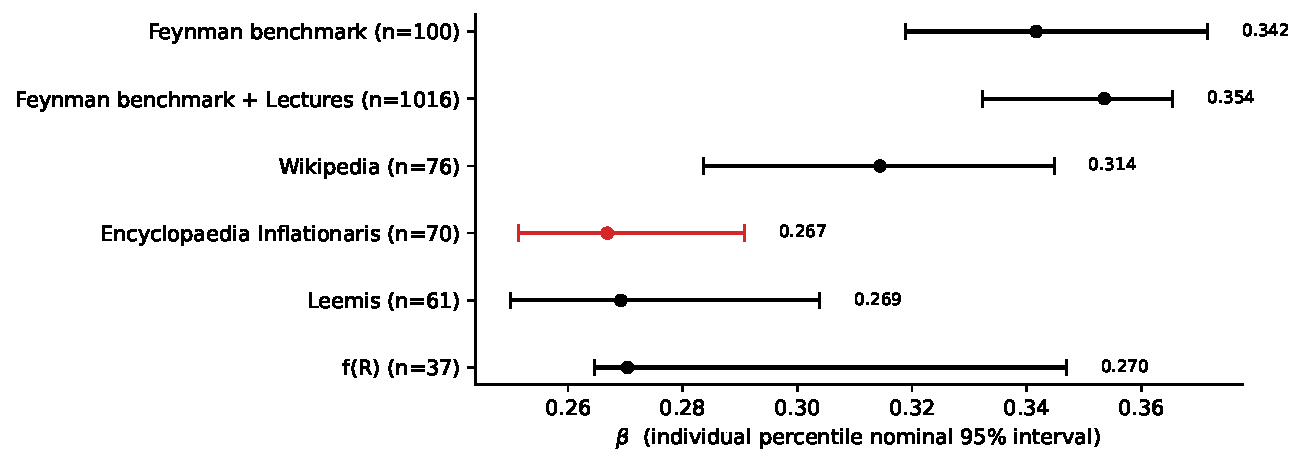
\includegraphics[width=0.8\linewidth]{beta_by_corpus.pdf}
\caption{Corpus estimates and nominal individual 95\% equation-bootstrap intervals.}\label{fig:corpus}
\end{figure}

\begin{table}[H]\centering\small
\resizebox{\linewidth}{!}{\begin{tabular}{lrrrrrr}\toprule
Branch & Expr. & Instances & Ranks & $\hat\beta$ & Boot.\ SE & Individual interval\\\midrule
\tabinput{generated/branch_table.tex}
\bottomrule\end{tabular}}
\caption{Branch estimates and nominal individual 95\% equation-bootstrap intervals.}\label{tab:branch}
\end{table}

Figure~\ref{fig:rf} shows the distributions underlying these estimates. Each branch is ranked separately, and both the observed operator types and their ordering can differ. The fitted rates describe how concentrated the ranked frequencies are; identifying the operators responsible for these patterns requires examining their identities separately.

\begin{figure}[H]\centering
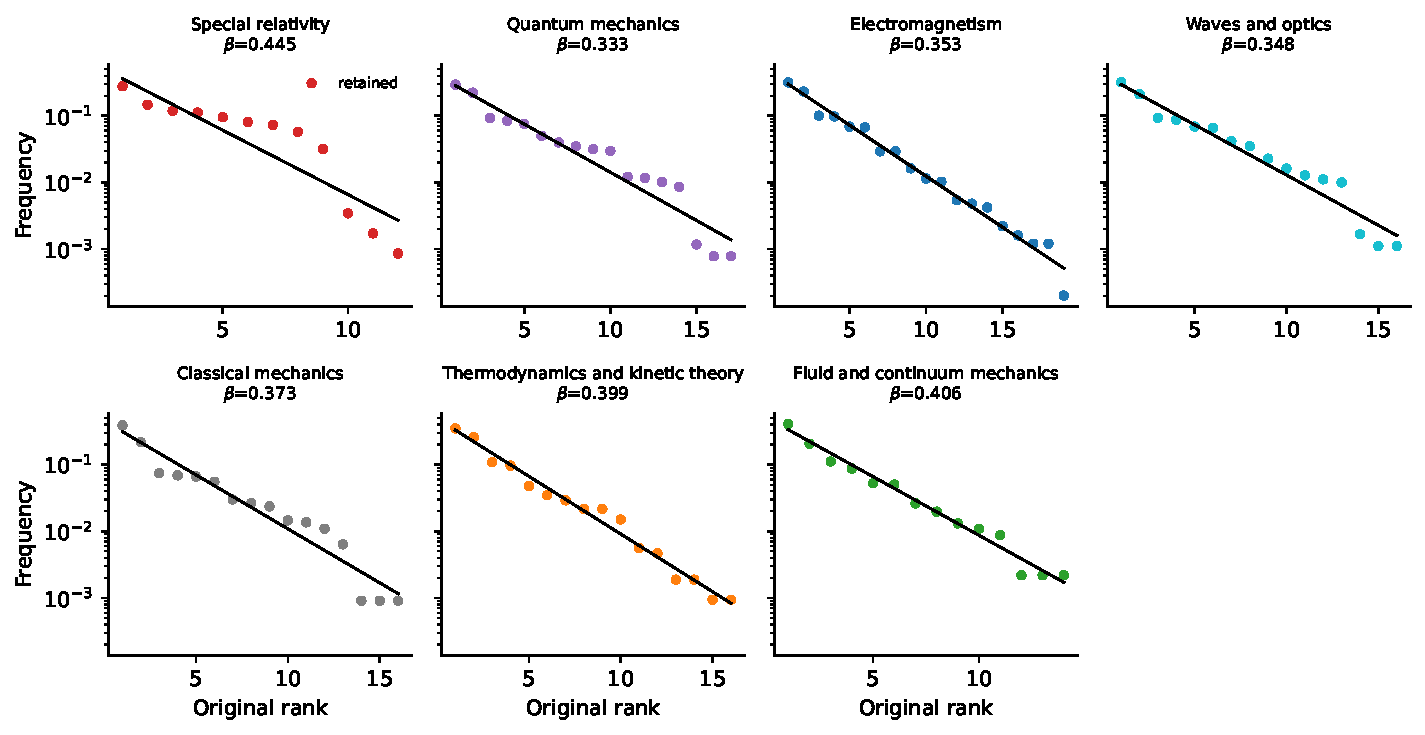
\includegraphics[width=\linewidth]{rank_frequency_branches.pdf}
\caption{Observed rank--frequency distributions and fitted exponentials for the seven branches.}\label{fig:rf}
\end{figure}

\subsection{Source-chapter resampling}
We resample whole chapters jointly across branches. For resampling, we place each chapter in a stratum using the most common Codex branch label among its retained equations. Ties follow the recorded branch order. Within each stratum, we sample the original number of chapters with replacement. Every equation from a selected chapter receives the same multiplicity, including equations assigned to other branches. This preserves dependence induced by the 54 chapters represented in more than one branch; the number of equations per branch can vary between replicates.

The individual chapter-bootstrap intervals are [0.355, 0.473] for fluid and continuum mechanics and [0.287, 0.365] for quantum mechanics. Both are wider than their equation-bootstrap intervals, and they overlap slightly.
\begin{figure}[H]\centering
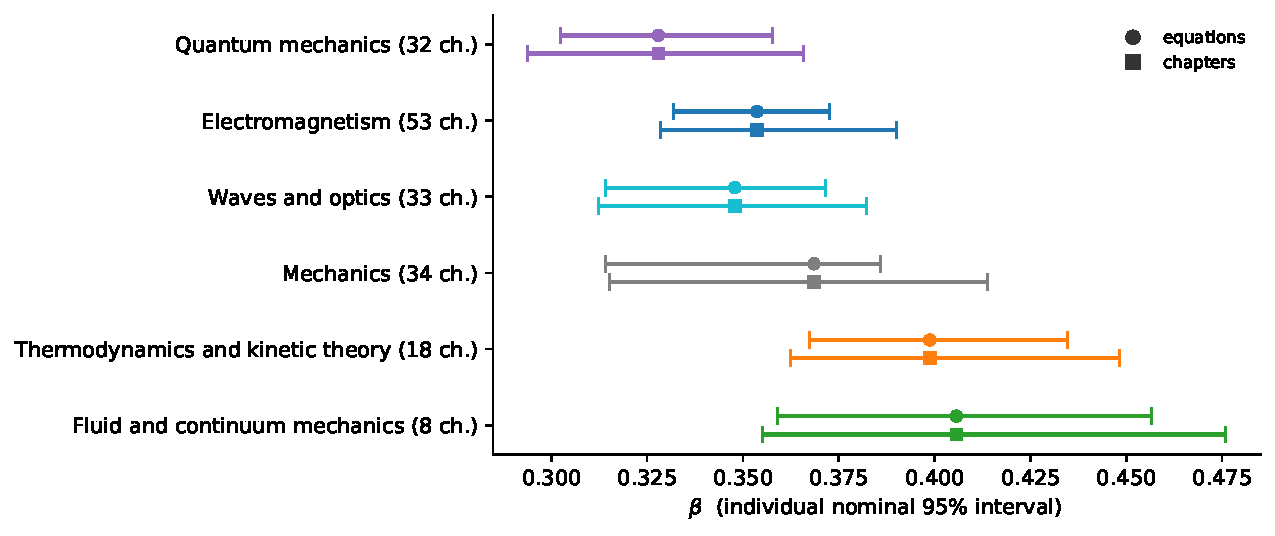
\includegraphics[width=0.85\linewidth]{chapter_bootstrap.pdf}
\caption{Equation and joint chapter bootstrap intervals at the nominal individual 95\% level. Labels give the number of source chapters represented in each branch.}\label{fig:chapter}
\end{figure}

\subsection{Branch assignments and selection}
We repeat the fits using only each formula's primary Codex label, excluding formulas flagged for averages or imaginary units, or excluding all formulas sourced from Volume~III. The last check uses the source references of both the lecture and benchmark formulas. Table~\ref{tab:assignment} reports the estimates and individual equation-bootstrap intervals.

\begin{table}[H]\centering\scriptsize
\begin{tabular}{llrrl}\toprule
Specification & Branch & Expr. & $\hat\beta$ & Individual interval\\\midrule
Primary Codex label only & SR & 83 & 0.442 & [0.326, 0.475] \\
 & QM & 211 & 0.313 & [0.278, 0.342] \\
 & EM & 296 & 0.336 & [0.323, 0.368] \\
 & Waves & 127 & 0.336 & [0.305, 0.362] \\
 & Classical & 113 & 0.367 & [0.306, 0.384] \\
 & Thermo & 89 & 0.392 & [0.361, 0.429] \\
 & Fluid & 48 & 0.405 & [0.362, 0.468] \\
\midrule
Notation-flagged expressions removed & SR & 87 & 0.445 & [0.330, 0.478] \\
 & QM & 170 & 0.318 & [0.292, 0.347] \\
 & EM & 379 & 0.355 & [0.336, 0.377] \\
 & Waves & 140 & 0.374 & [0.336, 0.399] \\
 & Classical & 108 & 0.373 & [0.322, 0.390] \\
 & Thermo & 92 & 0.397 & [0.365, 0.433] \\
 & Fluid & 51 & 0.405 & [0.358, 0.467] \\
\midrule
Volume III expressions removed & SR & 83 & 0.461 & [0.311, 0.480] \\
 & QM & 43 & 0.377 & [0.341, 0.436] \\
 & EM & 403 & 0.342 & [0.330, 0.369] \\
 & Waves & 146 & 0.343 & [0.311, 0.367] \\
 & Classical & 113 & 0.369 & [0.311, 0.381] \\
 & Thermo & 92 & 0.394 & [0.363, 0.431] \\
 & Fluid & 54 & 0.406 & [0.360, 0.458] \\
\bottomrule\end{tabular}
\caption{Sensitivity to label selection and formula inclusion. Each entry reports the fitted rate and its nominal individual 95\% equation-bootstrap interval. Waves denotes waves and optics. Fluid denotes fluid and continuum mechanics.}\label{tab:assignment}
\end{table}

\section{Bootstrap calibration}\label{app:calibration}
A 95\% interval should contain the true decay rate about 95 times in 100 repetitions. To check this, we generate data with a known rate, fit each dataset, and count how often the bootstrap interval includes that rate. We generate 200 datasets in each of three scenarios. Each dataset has seven groups of equations, and we use 400 bootstrap replicates to calculate the intervals. All scenarios have population marginal operator frequencies following an exponential with rate $\beta=0.35$. The first uses identical distributions and independent equation count vectors. The second varies equation counts, operator vocabularies and expression lengths, with dependence within an equation introduced through a shared random probability vector. The third introduces a shared random probability vector within each chapter and resamples whole chapters, including a branch with only four chapters.

Across the seven groups, the intervals included the true rate between 170 and 189 times out of 200 when we resampled equations, and between 149 and 169 times when we resampled chapters. Coverage fell below the nominal 95\% level, with the largest shortfall in the chapter-dependent scenario. We also recorded failed fits. These results describe simulations of operator counts and give an indication of how the reported intervals can behave.

\section{Exponential limit of the Zipf--Mandelbrot distribution}\label{app:zipf-limit}
For a fixed set of ranks $r=1,\ldots,R$, the normalised Zipf--Mandelbrot distribution is
\begin{equation}
p_r(\alpha,b)=\frac{(r+b)^{-\alpha}}{\sum_{s=1}^{R}(s+b)^{-\alpha}},
\qquad \alpha>0,\quad b>0.
\end{equation}
An exponential distribution is obtained when $b\to\infty$ and $\alpha/b\to\beta>0$. To see this, cancel the common factor $b^{-\alpha}$ from the numerator and denominator:
\begin{equation}
p_r(\alpha,b)=\frac{\exp[-\alpha\log(1+r/b)]}{\sum_{s=1}^{R}\exp[-\alpha\log(1+s/b)]}.
\end{equation}
Since $R$ is fixed, the expansion
\begin{equation}
\alpha\log(1+r/b)=\frac{\alpha}{b}r+O\!\left(\frac{\alpha R^2}{b^2}\right)
\end{equation}
holds uniformly over the ranks. Under the specified scaling, the remainder tends to zero and hence
\begin{equation}
p_r(\alpha,b)\longrightarrow\frac{e^{-\beta r}}{\sum_{s=1}^{R}e^{-\beta s}},
\end{equation}
recovering Eq.~\eqref{eq:law}. The scaling of both parameters matters: if $b$ increases while $\alpha$ is held fixed, the limiting distribution is uniform, $p_r\to1/R$.

This limiting relationship helps interpret comparisons of the Zipf--Mandelbrot and exponential models. Whether fitted parameters for a particular corpus approach this regime requires examining their values relative to the observed rank range. The limiting argument alone makes no claim about the empirical preference between the models.

\section{Prior fitting and sensitivity checks}\label{app:prior-fitting}

One component, $P_{\mathrm{geom},d}$, takes the ratio of the shallow branch and pooled probabilities, raises it to the power $0.15$, and uses it to adjust the deeper pooled probabilities before normalising within each context. In each outer training set, three further group-based folds supply the validation predictions used to fit the mixture weights. We estimate the weights on validation predictions within the training set, giving each training family equal weight in the validation objective and regularising toward the pooled model. The fixed 25\% share comes from exploratory comparisons on this corpus.

As a sensitivity check, we train and evaluate with only each expression's primary Codex label. On the same 943 formulas and six folds, this gives an overall probability ratio of 1.42.

\subsection{Averaging probabilities across branches}\label{app:prior-probability-mixture}
When all branch labels of an expression are supplied together, we can average the probabilities from the corresponding priors,
\begin{equation}
P_{\mathrm{mix}}(g_i)=\frac{1}{|B_i|}\sum_{b\in B_i}P_b(g_i).
\end{equation}
The geometric mean of $P_{\mathrm{mix}}(g_i)/P_{\mathrm{pool}}(g_i)$ over the same 943 expressions is 1.41. This aggregation takes the arithmetic mean of the branch probabilities within each expression. It is at least as large as their geometric mean, which is the quantity used in the main comparison.

\end{document}
